% Created 2019-04-16 Tue 22:54
% Intended LaTeX compiler: pdflatex
\documentclass[11pt]{article}
\usepackage[utf8]{inputenc}
\usepackage[T1]{fontenc}
\usepackage{graphicx}
\usepackage{grffile}
\usepackage{longtable}
\usepackage{wrapfig}
\usepackage{rotating}
\usepackage[normalem]{ulem}
\usepackage{amsmath}
\usepackage{textcomp}
\usepackage{amssymb}
\usepackage{capt-of}
\usepackage{hyperref}
\usepackage{float}
\topmargin 0mm \oddsidemargin 2mm \evensidemargin 2mm \textwidth 160mm \textheight 578.201 pt
\author{Guido España}
\date{\today}
\title{Cost-effectiveness of Dengvaxia in Puerto Rico}
\hypersetup{
 pdfauthor={Guido España},
 pdftitle={Cost-effectiveness of Dengvaxia in Puerto Rico},
 pdfkeywords={},
 pdfsubject={},
 pdfcreator={Emacs 26.1 (Org mode 9.1.9)}, 
 pdflang={English}}
\begin{document}

\maketitle

\section{Introduction}
\label{sec:orgf018ca5}
The latest results of the CYD-TDV vaccine show an increased risk of severe dengue upon infection among vaccinees without previous exposure to dengue virus (DENV) \cite{Sridhar2018}. The World Health Organization (WHO) recommends a pre-vaccination screening to ensure that only those with previous exposure to DENV are vaccinated \cite{WHO2018}. However, rapid diagnostic tests with high sensitivity and specificity are not currently available. We have previously discussed the benefits and cost-effectiveness of pre-screening vaccination for economic scenarios of the Philippines and Brazil \cite{Espana2019Biorxiv}. Here, we discuss the implications of this strategy for Puerto Rico in terms of epidemiological benefits and cost-effectiveness. 

\section{Methods}
\label{sec:org904a131}
We updated our assumptions of treatment of dengue for ambulatory cases and hospitalizations, based on estimates from 2002 to 2010 \cite{Halasa2012}. Using the consumer price index for Puerto Rico, we projected these costs to 2019 USD. Similarly, we took the GDP per-capita for Puerto Rico in 2016 \cite{worldbank2016} and projected it's value to 2019. 

\begin{center}
\begin{tabular}{llr}
\hline
 & Cost (USD) & Cost Projected (2019 USD)\\
\hline
Ambulatory & 239 (2010) & 311\\
Hospitalization & 1615 (2010) & 2107\\
GDP per-Capita & 30,833 (2016) & 30,833\\
\hline
\end{tabular}
\end{center}

We estimated the quality-adjusted life-years (QALY) gained with the pre-vaccination screening using disability weights and the time of disability from previous studies \textbf{(\url{SHIM} or someoneelse)}. We assumed a weight of 1 to estimate the QALYs gained from deaths averted. Similar to other studies (REFs), we used a discounting weight of 3\% per year for future cases, and we adjusted for life-expectancy using a discounting rate of 3\% as well. 

\begin{center}
\begin{tabular}{lrl}
\hline
Event & Disability weight & Time of disability\\
\hline
Dengue fever & 0.0158 & 4 days\\
Hospitalization & 0.545 & 14 days\\
Deaths & 1 & Life-expectancy - age of death\\
\hline
\end{tabular}
\end{center}

We then calculated the Incremental Cost-Effectiveness Ratio (ICER) as in equation \ref{eq-ICER}. As others have, we deemed the intervention cost-effective if the ICER was below 3 GDP per-Capita, and very cost-effective if the ICER fell below 1 GDP per-Capita. We assumed a baseline scenario of costs.

\begin{equation}
     ICER = \frac{Cost_{intervention} - Cost_{no-intervention}}
     {QALY_{intervention} - {QALY_{no-intervention}}}
     \label{eq-ICER}
\end{equation}

\section{Results}
\label{sec:org117728a}
\subsection{Epidemiological benefits from vaccination}
\label{sec:org3ba44c7}
The benefits are outlined in Figure 

\begin{figure}[htbp]
\centering
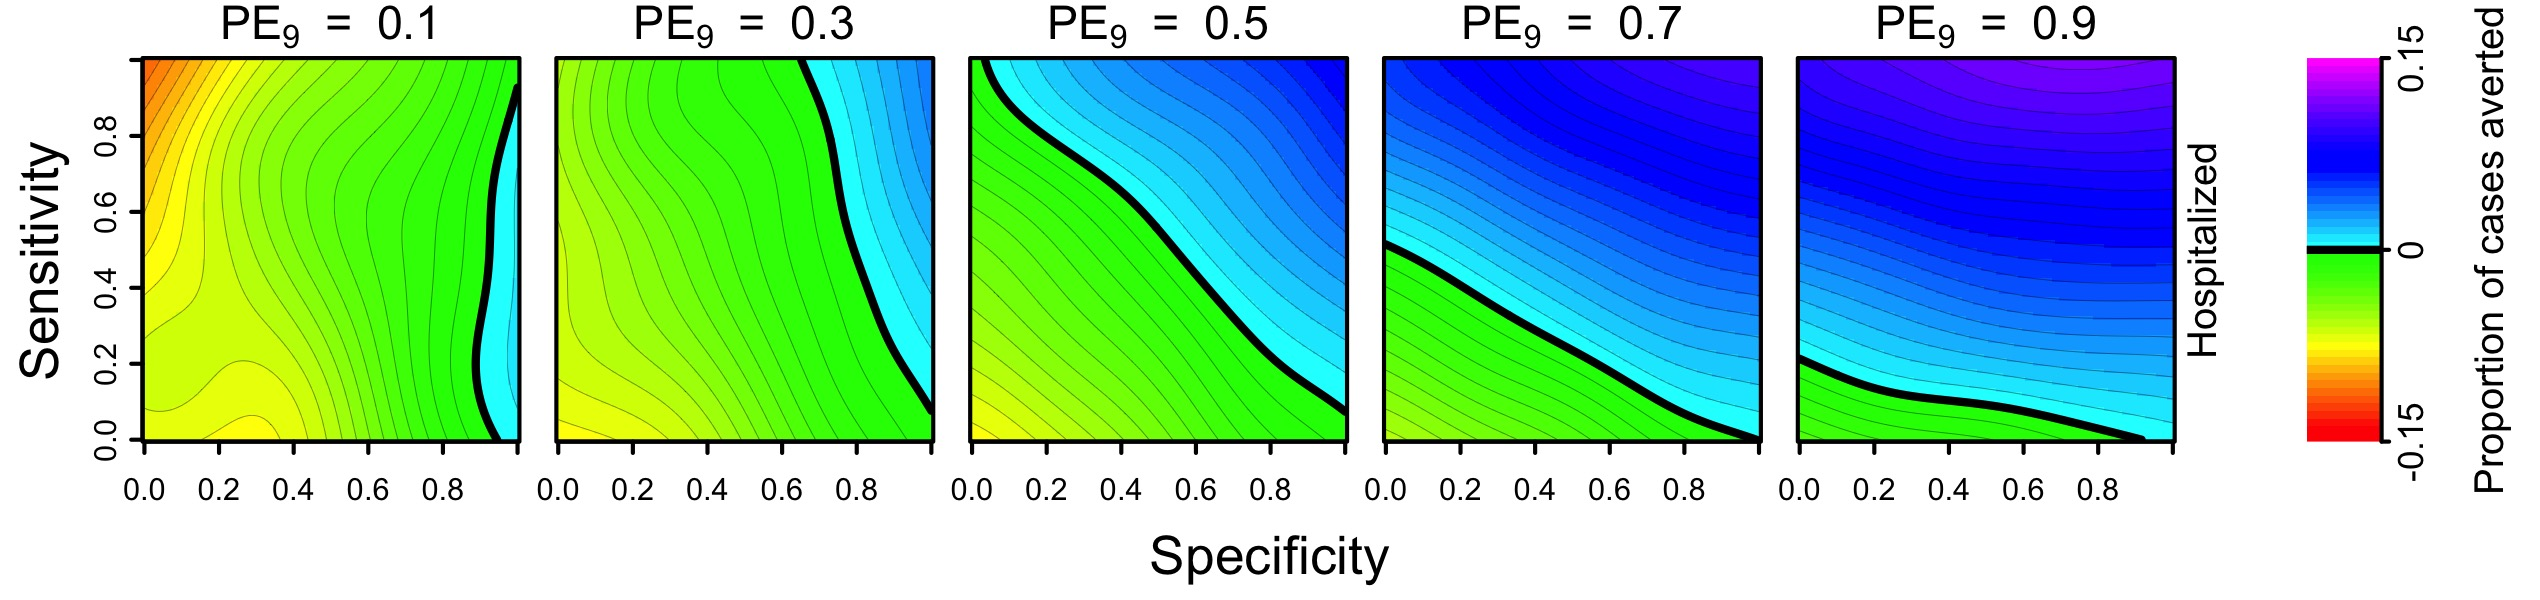
\includegraphics[width=.9\linewidth]{./figures/report_figure_cases_averted_heatmap_10y.jpeg}
\caption{\label{fig:org1e3c6d2}
Proportion of cases averted with pre-vaccination screening strategy with CYD-TDV over 10 years}
\end{figure}

\subsection{Cost-effectiveness of pre-vaccination screening strategies}
\label{sec:org3260f26}
Out cost-effectiveness analysis suggests that the intervention would be cost-effective in Puerto Rico at the assumed price of the vaccine (70 USD) (Fig. \ref{fig-ICER}). Below 200 USD per fully vaccinated person, pre-vaccination screening would be cost-effective from a public payer perspective (ICER < 3 GDP per Capita). Very cost-effective scenarios could be achieved with a vaccine price below 95 USD per vaccinated individual. Also, at 18 USD per vaccinated individual, the costs of the intervention are equal to the costs without intervention (ICER = 0). Nonetheless, these cost-effectiveness thresholds depend on our assumptions of specificity and sensitivity of screening. 

\textbf{An alternative scenario of low sensitivity shows that the cost-effectiveness is slightly reduced. We found similar results for a scenario with low specificity.} 


\begin{figure}[H]
\centering \includegraphics[width=.7\linewidth]{./figures/report_figure_ICER_PublicPayer_PuertoRico_10y.jpeg}
\label{fig-ICER}
\caption{ICER of pre-vaccination screening strategy in Puerto Rico at different cost of vaccination (3 doses per person).} 
\end{figure}

\subsection{Tornado diagram and sensitivity analysis}
\label{sec:org0147e73}
We varied the baseline value of five parameters of the cost-effectiveness analysis: sensitivity, specificity, PE9, vaccine cost for a fully vaccinated individual, and screening unit cost. The ranges of the parameter values are summarized in table \ref{table-tornado}. Compared to the sensitivity of screening, the specificity showed a larger impact in the cost-effectiveness of the intervention (Figure \ref{fig-tornado}). The lowest assumption of this parameter (0.5) resulted in an ICER above four time the GDP per Capita of Puerto Rico. In contrast, the same value for the sensitivity of screening yielded an ICER slightly above one GDP per Capita. We also found that a lower transmission intensity (50\% below baseline) than what we have assumed would affect the cost-effectiveness of the intervention more than a higher transmission intensity (50\% above baseline). Finally, a higher cost of the screening test (50 USD) would still result in ICER values below three GDP per Capita, and the vaccine cost could be up to 250 USD for ICER values below three GDP per Capita. 


\begin{figure}[H]
\centering 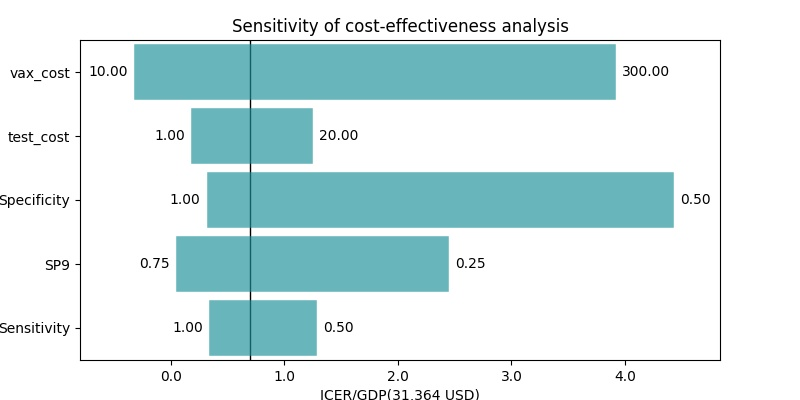
\includegraphics[width=.8\linewidth]{./figures/report_figure_tornado_diagram.jpeg}
\label{fig-tornado}
\caption{ICER of pre-vaccination screening strategy in Puerto Rico at different cost of vaccination (3 doses per person).} 
\end{figure}

\section{Discussion}
\label{sec:org6db2042}
Using an agent-based model of dengue transmission, we simulated the impact of a pre-vaccination screening strategy for 10 years of routine vaccination at different levels of transmission. Our model has been previously calibrated to represent longitudinal data of dengue transmission in Peru. This model has also been used in assessments of vaccination impact with CYD-TDV \cite{flasche2016}. Assuming a moderate transmission intensity (PE\(_{\text{9}}\) = 0.5) in Puerto Rico, we found that this intervention could be beneficial from the public health and individual perspective, conditioned to moderate values of sensitivity and high values of specificity. Compared to our previous simulation analysis for the Philippines and Brazil \cite{Espana2019Biorxiv}, the main differences of this analysis are the costs of treatment of dengue fever and severe dengue cases, which are based on studies from 2010. More recent estimates of this type of costs would refine the estimates of cost-effectiveness of pre-vaccination screening with CYD-TDV in Puerto Rico. 

\bibliographystyle{vancouver}
\bibliography{../../../../../Literature/Guido_Postdoc_Literature}
\end{document}